\documentclass[a4paper,12pt,nogin]{article}
%\VignetteIndexEntry{Manual for the chroGPS library}
%\VignettePackage{chroGPS}

\usepackage{amsmath}    % need for subequations
\usepackage{amssymb}    %useful mathematical symbols
\usepackage{bm}         %needed for bold greek letters and math symbols
\usepackage{graphicx}   % need for PS figures
%\usepackage{verbatim}   % useful for program listings
\usepackage{color}      % use if color is used in text
\usepackage{hyperref}   % use for hypertext links, including those to external documents and URLs
\usepackage{natbib}    %number and author-year style referencing
%\usepackage{epsf} 
%\usepackage{lscape} 
%\bibpunct{(}{)}{;}{a}{,}{,}
\usepackage[hmargin=3.5cm,vmargin=3cm]{geometry}
\newcommand{\newtext}[1]{{\color{blue} #1}} %Use \newtext{This is new text}
\newcommand{\drcomment}[1]{{\color{red} #1}} %Use \drcomment{This is a comment}

%\pagestyle{empty} % use if page numbers not wanted

 % Keep code 'as is'

\usepackage{Sweave}
\begin{document}

\title{\texttt{chroGPS}: visualizing the epigenome. }
\small
\author{Oscar Reina \footnote{Bioinformatics \& Biostatistics Unit,
    IRB Barcelona}  and David Rossell
  \footnotemark[1] }
\normalsize
\date{}  %comment to include current date

\maketitle


\section{Introduction}
\label{sec:intro}

The \texttt{chroGPS} package provides tools to generate intuitive maps to visualize the association between genetic elements, with emphasis on epigenetics. The approach is based on Multi-Dimensional Scaling. We provide several sensible distance metrics, and adjustment procedures to remove systematic biases typically observed when merging data obtained under different technologies or genetic backgrounds.
\newtext{This manual illustrates the software functionality and highlights some ideas,
for a detailed technical description the reader is referred to (our paper, Supplementary Material).}
\\\\
Many routines allow performing computations in parallel 
by specifying an argument \texttt{mc.cores}, which uses
packages \texttt{multicore} \newtext{and \texttt{parallel}.
These packages are not available under Windows, so here we call the functions with a single processor (the default option).}
%As this package makes extensive use of the multicore library, we will
%load it to ensure parallel computation is available with our 4
%available cores. You shoud adequate
%this to your system: the default option for all functions is use a
%single processor, but you can also force that by using mc.cores=1 in
%the function calls if you want.
Please see the help page for each function for more details.
\\\\
We start by loading the package and a ChIP-chip dataset with genomic
distribution of 20 epigenetic elements from the Drosophila melanogaster
S2-DRSC cell line, coming from the modEncode project, which we will use for illustration purposes.
Even though our study and examples focuses on assessing associations
between genetic elements, this methodology can be successfully used with
any kind of multivariate data where relative distances between
elements of interest can be computed based on a given set of variables.

\section{chroGPS-factors}
\label{sec:chrogps_factors}

\footnotesize

\begin{Schunk}
\begin{Sinput}
> options(width=70)
> library(chroGPS)
> data(s2)
> s2
\end{Sinput}
\begin{Soutput}
RangedDataList of length 20
names(20): ASH1-Q4177.S2 CP190-HB.S2 ... Su(var)3-9.S2 mod2.2-VC.S2
\end{Soutput}
\end{Schunk}

\normalsize

\texttt{s2} is a \texttt{RangedDataList} object storing the
binding sites for 20 Drosophila melanogaster S2-DRSC sample
proteins. Data was retrieved from the modEncode website
(www.modencode.org) and belongs to the public subset of the Release 29.1 dataset. GFF files
were downloaded, read and formatted into individual RangedData
objects, stored later into a \texttt{RangedDataList} (see functions \texttt{getURL} and 
\texttt{gff2RDList} for details.)
 
 
\subsection{Building chroGPS-factors maps}
\label{ssec:factormaps}
 
The methodology behing chroGPS-factors is to generate a distance
matrix with all the pairwise distances between elements of interest by
means of a chosen metric. After this, a Multidimensional Scaling
representation is generated to fit the n-dimensional distances in a
lower (usually 2 or 3) k-dimensional space.
 
\footnotesize
 
\begin{Schunk}
\begin{Sinput}
> d <- distGPS(s2, metric='avgdist')
> d
\end{Sinput}
\begin{Soutput}
Object of class distGPS with avgdist distances between 20 objects 
\end{Soutput}
\begin{Sinput}
> mds1 <- mds(d,k=2,type='isoMDS')
> mds1
\end{Sinput}
\begin{Soutput}
Object of class MDS approximating distances between 20 objects 
R-squared= 0.6284 Stress= 0.0795 
\end{Soutput}
\begin{Sinput}
> mds1.3d <- mds(d,k=3,type='isoMDS')
> mds1.3d
\end{Sinput}
\begin{Soutput}
Object of class MDS approximating distances between 20 objects 
R-squared= 0.8577 Stress= 0.0287 
\end{Soutput}
\end{Schunk}
 
\normalsize
 
The R$^2$ coefficient between the original distances and their approximation in the
plot 
can be seen as an analogue to the percentage of explained variability in a PCA analysis.
For our sample data R$^2$=0.628
%(up to rounding), 
\newtext{and stress=0.079 in the 2-dimensional plot, both of which}
indicate a fairly good fit. A 3-dimensional plot improves these
values.
%even if it is not necessarily easier to interpret without movement.
\newtext{We can produce a map by using the \texttt{plot} method for \texttt{MDS} objects.
The result in shown in Figure \ref{fig:mds1}.
For 3D representations the \texttt{plot} method opens an interactive window
that allows to take full advantage of the additional dimension.
Here we commented out the code for the 3D plot and simply show a snapshot in Figure \ref{fig:mds1}.}

\drcomment{Explain where s2names.color comes from (saved as part of s2, what do they mean)}.

\footnotesize
 
\begin{Schunk}
\begin{Sinput}
> cols <- as.character(s2names$Color)
> plot(mds1,drawlabels=TRUE,point.pch=20,point.cex=8,text.cex=.7,
+ point.col=cols,text.col='black',labels=s2names$Factor)
> legend('topleft',legend=sprintf('r2=%.3f',mds1@R.square),bty='n',cex=2)
> #plot(mds1.3d,drawlabels=TRUE,type.3d='s',point.pch=20,point.cex=.1,text.cex=.7,
> #point.col=cols,text.col='black',labels=s2names$Factor)
\end{Sinput}
\end{Schunk}

\normalsize

\setkeys{Gin}{width=0.8\textwidth} 
\begin{figure}
\begin{center}
\includegraphics{chroGPS-figmds1}
{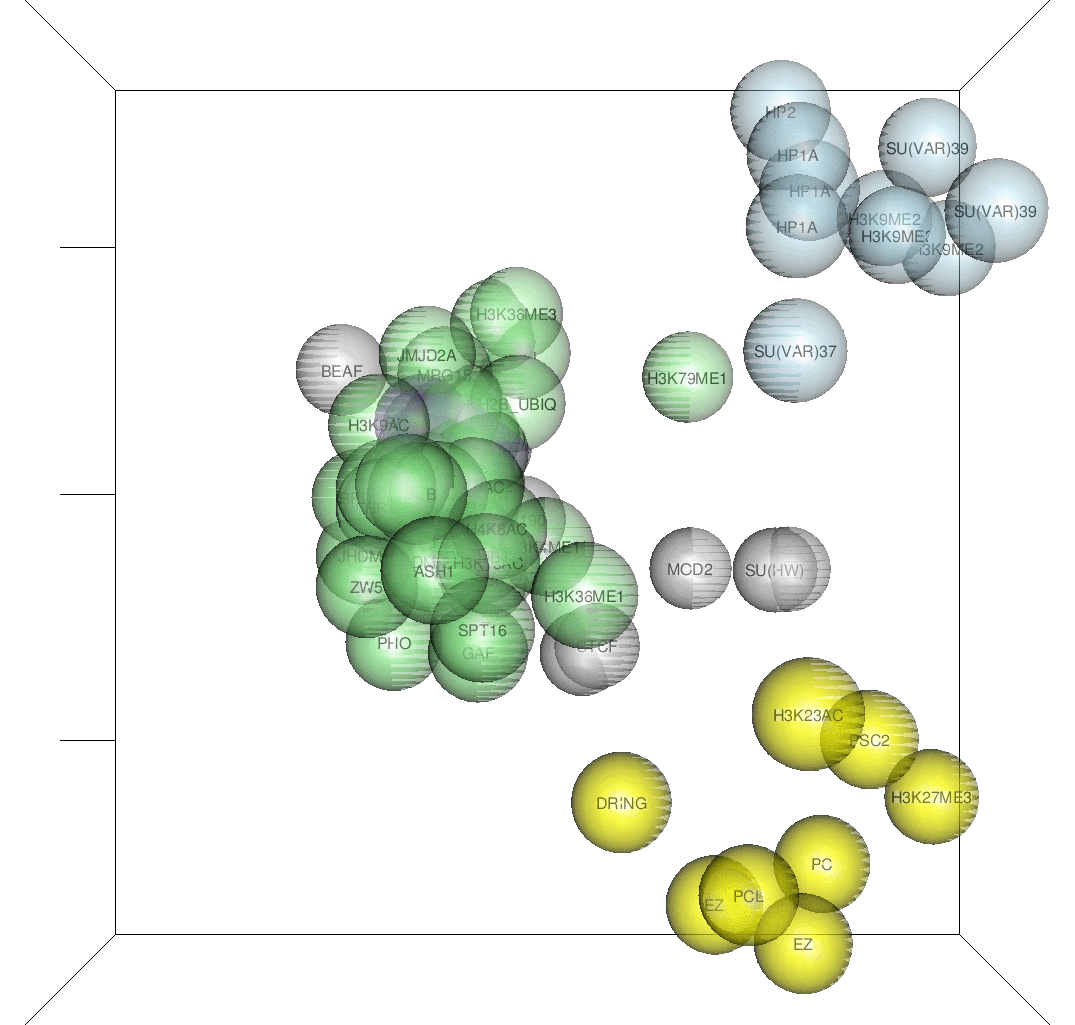
\includegraphics{mds3d_1.png}}
\end{center}
\caption{2D and 3D MDS maps from the 20 S2 epigenetic factors. Factors with more similar binding site distribution appear closer}
\label{fig:mds1}
\end{figure}
 
 
\subsection{Integrating data sources: technical background}
\label{ssec:tecbias}
 
Currently, genomic profiling of epigenetic factors is being largely
determined through high throughput methodologies such as
ultra-sequencing (ChIP-Seq), which identifies binding sites with higher
accuracy that ChIP-chip 
\newtext{experiments. However,}
%data, even though 
there is an extensive
knowledge background based on the later. ChroGPS allows
integrating different technical sources by adjusting for
systematic biases.
\\\\
We propose two adjustment methods: Procrustes and Peak Width 
Adjustment. Procrustes finds the optimal superimposition of two sets of
points by altering their location, scale and orientation while
maintaining their relative distances. It is therefore a
general method of adjustment that can take care of several kind of
biases. However, its main limitation is that a minimal set of common
points (that is, the same factor/protein binding sites mapped in both data sources) is needed to effectively perform a valid adjustment. Due to the spatial nature of Procrustes adjustment, we strongly recommend a minimum number of 3 common points.

\newtext{We illustrate the adjustments by loading {\it Drosophila melanogaster} S2 ChIP-seq data obtained from} \drcomment{...}
\newtext{We start by producing a joint map with no adjustment.}

\drcomment{I only see 3 ChIP-seq points in the map, but there are supposed to be 4.}

\footnotesize
 
\begin{Schunk}
\begin{Sinput}
> data(s2Seq)
> s2Seq
\end{Sinput}
\begin{Soutput}
RangedDataList of length 4
names(4): GSM480156_dm3-S2-H3K4me3.bed.rd ...
\end{Soutput}
\begin{Sinput}
> d2 <- distGPS(c(s2,s2Seq),metric='avgdist')
> mds2 <- mds(d2,k=2,type='isoMDS')
> cols <- c(as.character(s2names$Color),as.character(s2SeqNames$Color))
> sampleid <- c(as.character(s2names$Factor),as.character(s2SeqNames$Factor))
> pchs <- rep(c(20,17),c(length(s2),length(s2Seq)))
> point.cex <- rep(c(8,5),c(length(s2),length(s2Seq)))
> plot(mds2,drawlabels=TRUE,point.pch=pchs,point.cex=point.cex,text.cex=.7,
+ point.col=cols,text.col='black',labels=sampleid)
> legend('topleft',legend=sprintf('r2=%.3f',mds2@R.square),bty='n',cex=1.5)
> legend('topright',legend=c('ChIP-Chip','ChIP-Seq'),pch=c(20,17),pt.cex=c(1.5,1))
\end{Sinput}
\end{Schunk}
 
\normalsize
 
\setkeys{Gin}{width=0.8\textwidth} 
\begin{figure}
\begin{center}
\begin{Schunk}
\begin{Soutput}
RangedDataList of length 4
names(4): GSM480156_dm3-S2-H3K4me3.bed.rd ...
\end{Soutput}
\end{Schunk}
\includegraphics{chroGPS-figprocrustes1}
\end{center}
\caption{S2 ChIP-chip and ChIP-Seq data, raw integration (no adjustment). }
\label{fig:procrustes1}
\end{figure}

\newtext{
Figure \ref{fig:procrustes1} shows the resulting map.
While ChIP-seq elements appear close to their ChIP-chip counterparts, they form an external layer.
We now apply Procrustes to adjust these systematic biases using function \texttt{procrustesAdj}.
}

\footnotesize
 
\begin{Schunk}
\begin{Sinput}
> adjust <- rep(c('chip','seq'),c(length(s2),length(s2Seq)))
> sampleid <- c(as.character(s2names$Factor),as.character(s2SeqNames$Factor))
> mds3 <- procrustesAdj(mds2,d2,adjust=adjust,sampleid=sampleid)
> plot(mds3,drawlabels=TRUE,point.pch=pchs,point.cex=point.cex,text.cex=.7,
+ point.col=cols,text.col='black',labels=sampleid)
> legend('topleft',legend=sprintf('r2=%.3f',mds3@R.square),bty='n',cex=1.5)
> legend('topright',legend=c('ChIP-Chip','ChIP-Seq'),pch=c(20,17),pt.cex=c(1.5,1))
\end{Sinput}
\end{Schunk}
 
\normalsize
 
\setkeys{Gin}{width=0.8\textwidth} 
\begin{figure}
\begin{center}
\includegraphics{chroGPS-figprocrustes2}
\end{center}
\caption{S2 ChIP-chip and ChIP-Seq data, Procrustes adjustment}
\label{fig:procrustes2}
\end{figure}
 
Peak Width Adjustment relies on the basic difference between the two
different sources of information used in our case, that is, the
resolution difference between ChIP-Seq and ChIP-chip peaks, which
translates basically in the width presented by the regions identified
as binding sites, being those peaks usually much wider in ChIP-chip
data (poorer resolution).
 
\footnotesize
 
\begin{Schunk}
\begin{Sinput}
> s2.pAdj <- adjustPeaks(c(s2,s2Seq),adjust=adjust,sampleid=sampleid,logscale=TRUE)
> d3 <- distGPS(s2.pAdj,metric='avgdist')
> mds4 <- mds(d3,k=2,type='isoMDS')
> plot(mds4,drawlabels=TRUE,point.pch=pchs,point.cex=point.cex,text.cex=.7,
+ point.col=cols,text.col='black',labels=sampleid)
> legend('topleft',legend=sprintf('r2=%.3f',mds4@R.square),bty='n',cex=1.5)
> legend('topright',legend=c('ChIP-Chip','ChIP-Seq'),pch=c(20,17),pt.cex=c(1.5,1))
\end{Sinput}
\end{Schunk}
 
\normalsize
 
\setkeys{Gin}{width=0.8\textwidth} 
\begin{figure}
\begin{center}
\includegraphics{chroGPS-figpeakwidth1}
\end{center}
\caption{S2 ChIP-chip and ChIP-Seq data, Peak Width Adjustment}
\label{fig:peakwidth1}
\end{figure}

\newtext{
Figure \ref{fig:peakwidth1} shows the map after Peak Width Adjustment,
where ChIP-chip and ChIP-seq elements have been adequately matched.
}
Whenever possible, we strongly recommend using Procrustes adjustment
due to its general nature and lack of 
%a-priori 
\newtext{mechanistic} assumptions. This is
even more important if integrating other data sources for binding
site discovery, such as DamID, Chiapet, etc, where technical biases
are more complex than just peak location resolution and peak size.
 
\subsection{Integrating data sources: biological background. Assessing
cellular conservation}
\label{ssec:biobias}

\drcomment{Aquesta seccio la treuria si necessitessim reduir temps de vignette, no expliquem cap funcionalitat nova i ja ho tenim al paper i suppl mat.}

Functional co-operation between epigenetic factors is largely
conserved in different cell types and tissues. Thus, it can be
anticipated that chroGPS-factors maps would reflect this. To address
this question we will use modEncode data from a different Drosophila
cell line, BG3, using several common factors with our S2 sample and
also some new ones. As with the S2 data, we will start by loading the dataset and building the chroGPS-factors map for it.
 
\footnotesize
 
\begin{Schunk}
\begin{Sinput}
> data(bg3)
> d2 <- distGPS(bg3,metric='avgdist')
> mds2 <- mds(d2,type='isoMDS')
> cols <- as.character(bg3names$Darkcolor)
> plot(mds2,drawlabels=TRUE,point.pch=20,point.cex=8,text.cex=.7,
+ point.col=cols,text.col='white',labels=bg3names$Factor)
> legend('topleft',legend=sprintf('r2=%.3f',mds2@R.square),bty='n',cex=2)
\end{Sinput}
\end{Schunk}
 
\normalsize
 
\setkeys{Gin}{width=0.8\textwidth} 
\begin{figure}
\begin{center}
\includegraphics{chroGPS-mds3}
\end{center}
\caption{chroGPS-factors map with 18 epigenetic elements from modEncode Dmelanogaster BG3 ChIP-chip data.}
\label{fig:mds3}
\end{figure}
 
When a novel factor from the same technical and biological
background (or even from different one) is fitted into an already well populated map, it is highly
unlikely that the new relative distances generated by this element
distort the map so much that it becomes unuseable. In fact, it can be
desirable to use this new distances to re-generate the map from
scratch, since this new information can help produce a more detailed
map where relationships between elements are defined by more evidences (as when creating geographical maps, new elements are what were used to integrate more detail into them).
 
\footnotesize
 
\begin{Schunk}
\begin{Sinput}
> d3 <- distGPS(c(s2,bg3),metric='avgdist',mc.cores=1)
> mds3 <- mds(d3,k=2,type='isoMDS')
> cols <- c(s2names$Color,bg3names$Darkcolor)
> textcols <- c(rep('black',length(s2)),rep('lightgrey',length(bg3)))
> plot(mds3,drawlabels=TRUE,point.pch=20,point.cex=8,text.cex=.7,
+ point.col=cols,text.col=textcols,labels=c(s2names$Factor,bg3names$Factor))
> legend('topleft',legend=sprintf('r2=%.3f',mds3@R.square),bty='n',cex=1.5)
\end{Sinput}
\end{Schunk}
 
\normalsize
 
A good example is a direct integration of SL2 and BG3 data which, without the need of any further adjustment, already produces a valid map with the conserved functional domains already seen in individual SL2 and BG3 maps. This is a by-product of an observed fact: actual overlap between common factors of different biological backgrounds is still higher than the overlap bewteen any given factors from the same biological backgrounds but from different functional domain. Therefore, functional domains are conserved.
 
\setkeys{Gin}{width=0.8\textwidth} 
\begin{figure}
\begin{center}
\includegraphics{chroGPS-mds4}
\end{center}
\caption{S2 (light) and BG3 (dark) ChIP-chip data, raw integration}
\label{fig:mds4}
\end{figure}
 
This domain conservation can be asessed with the \texttt{domainDist}
function, which computes inter or intra domain distances for a given
map. Since our domains are identified by factor color, we will use
that information for the domain distance calculation.
\\\\
First, we identify domains for each cellular background using factor colors which are already available.

\footnotesize
 
\begin{Schunk}
\begin{Sinput}
> adjust <- rep(c('s2','bg3'),c(length(s2),length(bg3)))
> domain.s2 <- s2names$Color
> domain.bg3 <- bg3names$Color
> domain.s2[domain.s2=='purple'] <- 'lightgreen'
> domain.bg3[domain.bg3=='purple'] <- 'lightgreen'
\end{Sinput}
\end{Schunk}

\normalsize
Now we compute inter and intra domain distances of interest with these color-based domains and the joint S2/BG3 map.

\footnotesize

\begin{Schunk}
\begin{Sinput}
> # Intra-domain S2
> intra.s2 <- domainDist(d3@d[adjust=='s2',adjust=='s2'],gps='factors',
+ domain=domain.s2,type='intra',avg=TRUE,col=c(sort(domain.s2),'white'),plot=FALSE)
> # Inter-domain S2
> inter.s2 <- domainDist(d3@d[adjust=='s2',adjust=='s2'],gps='factors',
+ domain=domain.s2,type='inter',avg=TRUE,plot=FALSE)
> # Intra-domain from joint map S2/BG3
> intra.s2.bg3 <- domainDist(d3@d[adjust %in% c('s2','bg3'),adjust %in% c('s2','bg3')],
+ gps='factors',domain=c(domain.s2,domain.bg3),type='intra',
+ avg=TRUE,col=c(sort(domain.s2),'white'),plot=FALSE)
> # Inter-domain from joint map S2/BG3
> inter.s2.bg3 <- domainDist(d3@d[adjust %in% c('s2','bg3'),adjust %in% c('s2','bg3')],
+ gps='factors',domain=c(domain.s2,domain.bg3),type='inter',
+ avg=TRUE,plot=FALSE)
> # Between-replicate S2/BG3 distances
> intra.s2.bg3.reps <- domainDist(d3@d[adjust %in% c('s2','bg3'),adjust %in% c('s2','bg3')],
+ gps='factors',domain=c(s2names$Factor,bg3names$Factor),
+ type='intra',avg=TRUE,col=c(sort(domain.s2),'white'),plot=FALSE)
\end{Sinput}
\end{Schunk}

\normalsize

And finally we can plot the resulting distances for inter and intra domain combinations.

\footnotesize

\begin{Schunk}
\begin{Sinput}
> labs <- c('S2/BG3 replicates','Intra-Domain S2','Inter-Domain S2',
+ 'Intra-Domain S2/BG3','Inter-Domain S2/BG3')
> cols <- rainbow(5,0.5)
> boxplot(intra.s2.bg3.reps$Avg,intra.s2$Avg,inter.s2$Avg,intra.s2.bg3$Avg,
+ inter.s2.bg3$Avg,ylim=c(0,1),notch=TRUE,xlim=c(0,10),col=cols)
> legend('topright',title='Distance (iOverlap)',legend=labs,bty='n',cex=1,
+ pch=19,pt.cex=2,col=cols,y.intersp=2,x.intersp=2)
\end{Sinput}
\end{Schunk}
 
\normalsize
 
\setkeys{Gin}{width=0.8\textwidth} 
\begin{figure}
\begin{center}
\includegraphics{chroGPS-domaindist1}
\end{center}
\caption{S2 and BG3 ChIP-chip data, individual and joint domain distance}
\label{fig:mds5}
\end{figure}
 
\section{ChroGPS-genes}
\label{ssec:genes}
 
In addition to assessing relationship between epigenetic factors,
chroGPS also provides tools to generate chroGPS-genes maps, useful to
visualize the relationships between genes based on their epigenetic
pattern similarities (the epigenetic marks they share).
 
\subsection{Building chroGPS-genes maps}
\label{ssec:genemaps}
 
The proceedings are analog to those of chroGPS-factors, that is, the
definition of a metric to measure similarity between genes and using
it to generate MDS representations in k-dimensional space. The data
source of chroGPS-genes has to be a matrix or data frame of N genes x
M factors (rows x cols), where each cell has a value of 1 if a binding
site for that protein or factor has been found in the region defined
by that gene. This annotation table can be generated by multiple
methods, in our case we annotated the genomic distribution on 76 S2
modEncode against the Drosophila melanogaster genome (Ensembl february 2012), accounting for
strict overlaps within 1000bp of gene regions. 
\drcomment{Indicate the function you used, R package and reference.}
After that, 500 random
genes were selected randomly and this is the dataset that will be used
in all further examples.
 
\footnotesize
 
\begin{Schunk}
\begin{Sinput}
> s2.tab[1:10,1:4]
\end{Sinput}
\begin{Soutput}
            ASH1-Q4177.S2 BEAF-70.S2 BEAF-HB.S2 Chro(Chriz)BR.S2
FBgn0051778             0          0          0                0
FBgn0028562             0          0          0                0
FBgn0011653             0          0          0                0
FBgn0262889             0          0          0                0
FBgn0030056             1          0          1                1
FBgn0035496             0          0          0                0
FBgn0026149             1          0          1                1
FBgn0030142             0          0          1                1
FBgn0003008             0          1          1                1
FBgn0052703             0          0          0                0
\end{Soutput}
\end{Schunk}
 
\footnotesize
 
\begin{Schunk}
\begin{Sinput}
> d <- distGPS(s2.tab, metric='tanimoto', uniqueRows=TRUE)
> d
\end{Sinput}
\begin{Soutput}
Object of class distGPS with tanimoto distances between 466 objects 
\end{Soutput}
\begin{Sinput}
> mds1 <- mds(d,k=2,type='isoMDS')
> mds1
\end{Sinput}
\begin{Soutput}
Object of class MDS approximating distances between 466 objects 
R-squared= 0.8217 Stress= 0.1269 
\end{Soutput}
\begin{Sinput}
> mds2 <- mds(d,k=3,type='isoMDS')
> mds2
\end{Sinput}
\begin{Soutput}
Object of class MDS approximating distances between 466 objects 
R-squared= 0.8884 Stress= 0.0757 
\end{Soutput}
\end{Schunk}
 
\normalsize
 
%As we increase the number of points, fitting a solution in
%k-dimensional spaces gets tougher. If desired, goodness-of-fit in
%terms of R$^2$ using the 
%\texttt{boostMDS} algorithm provided in our package. As can be seen,
Increasing k \newtext{improves the R$^2$ and stress values. 
For our examples here we use non-metric isoMDS by indicating \texttt{type='isoMDS'}, which calls}
% also makes for an improved fit. During all our examples, the base 
%MDS type used for chroGPS-genes maps will be the non-metric isoMDS one, as implemented in 
the \texttt{isoMDS} function from the
\texttt{MASS} package.
\drcomment{Add reference.}

\footnotesize
 
\begin{Schunk}
\begin{Sinput}
> plot(mds1,point.cex=1.5,point.col=densCols(mds1@points))
> #plot(mds2,point.cex=1.5,type.3d='s',point.col=densCols(mds2@points))
\end{Sinput}
\end{Schunk}
 
\normalsize
 
\setkeys{Gin}{width=1.0\textwidth} 
\begin{figure}
\begin{center}
{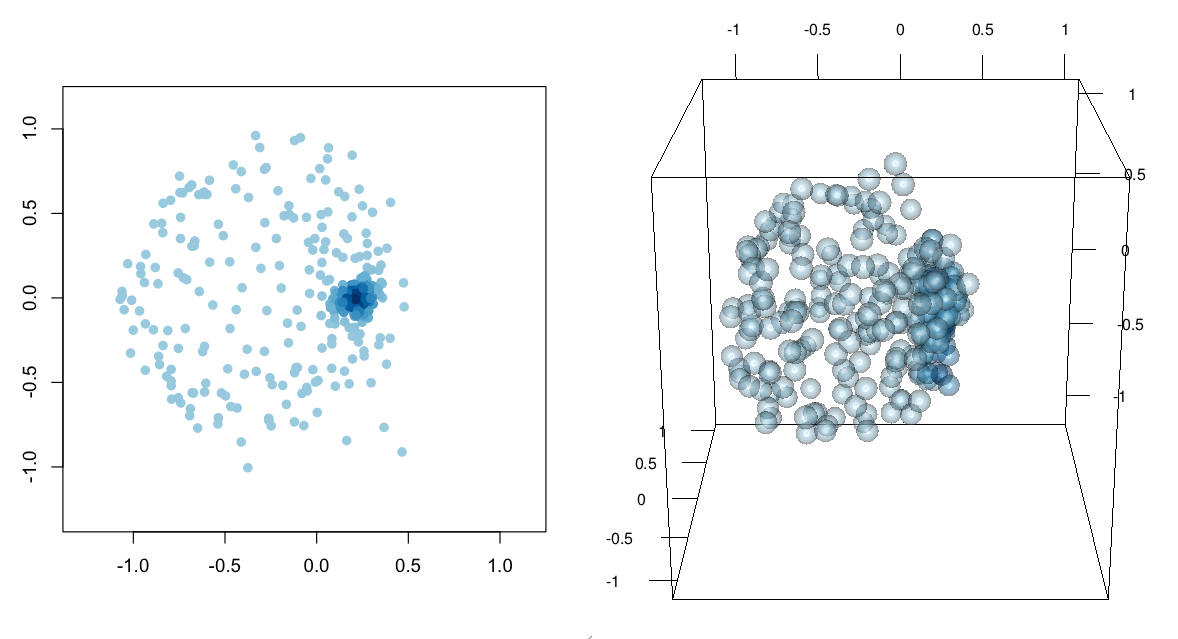
\includegraphics{mds-2d-3d.png}}
\end{center}
\caption{2 and 3-dimensional chroGPS-genes. Genes with more similar
  epigenetic marks (binding site patterns) appear closer.}
\label{fig:mds6}
\end{figure}
 
\subsection{Genome-wide chroGPS-genes maps}
\label{sec:splitMDS}
 
As mentioned, our example dataset for chroGPS-genes maps consists in a combination
of 76 protein binding sites for 500 genes. When only unique factor
combinations are considered (all genes sharing a specific combination
of epigenetic marks are merged into a single 'epigene'), the size of
the dataset gets down to 466 genes per 76 factors.
 
\footnotesize
 
\begin{Schunk}
\begin{Sinput}
> dim(s2.tab)
\end{Sinput}
\begin{Soutput}
[1] 500  76
\end{Soutput}
\begin{Sinput}
> dim(uniqueCount(s2.tab))
\end{Sinput}
\begin{Soutput}
[1] 466  78
\end{Soutput}
\end{Schunk}
 
\normalsize
 
However, when genome-wide patterns are considered, the number of epigenes can still be very high, in the order of ten
thousand unique epigenes. This poses a real challenge for
Multidimensional Scaling when trying to find an
optimal solution for k-space representation of the pairwise distances
\newtext{both in terms of accuracy and computational cost.}
%between all epigenes, but specially in terms of computing requirements
%(read memory and CPU time). Multidimensional Scaling is a classic
%example of an atomic task, therefore not suitable for problem
%subdivision and parallel computation. Some strategies, however,
%started to address this problem.
%% COMMENT: not really an atomic task if we managed to split it.

\newtext{We start by re-running the isoMDS fit and measuring the CPU time.}

\footnotesize
\begin{Schunk}
\begin{Sinput}
> system.time(mds3 <- mds(d,k=2,type='isoMDS'))
\end{Sinput}
\begin{Soutput}
   user  system elapsed 
  6.525   0.033   6.557 
\end{Soutput}
\begin{Sinput}
> mds3
\end{Sinput}
\begin{Soutput}
Object of class MDS approximating distances between 466 objects 
R-squared= 0.8217 Stress= 0.1269 
\end{Soutput}
\end{Schunk}
\normalsize

\newtext{We now apply our BoostMDS algorithm, which is a 2-step procedure}
%Using a divide-and-conquer approach 
(see package help for function \texttt{mds} for details).
\newtext{BoostMDS} 
%we are able to 
generates maps at much lower time and memory consumption requirements, 
\newtext{while improving the R$^2$ and stress coefficients}.
%with a R$^2$ correlation roughly equal to that of the traditional version. 
%The base of our approach is to
\newtext{The first step is to obtain an initial solution by} randomly splitting the original distance matrix in a number of smaller submatrices with a certain number of overlapping elements between them, so that individual MDS representations can be found for each one and later become stitched by using Procrustes with their common points. 
\newtext{The second step is to formally maximize the R$^2$ coefficient by using a gradient descent algorithm using the \texttt{boostMDS} function. The second step also ensures that the arbitrary split used in the first step does not have}
%Additionally, the resulting MDS can be further optimized with our boostMDS function. This 
%also ensures that the resampling used to split the original distance matrix is not having 
a decisive effect
on the final MDS point configuration.


\footnotesize
\begin{Schunk}
\begin{Sinput}
> system.time(mds3 <- mds(d,type='isoMDS',splitMDS=TRUE,split=.5,overlap=.05,mc.cores=1))
\end{Sinput}
\begin{Soutput}
   user  system elapsed 
  1.890   0.039   1.929 
\end{Soutput}
\begin{Sinput}
> mds3
\end{Sinput}
\begin{Soutput}
Object of class MDS approximating distances between 466 objects 
R-squared= 0.8002 Stress= 0.1301 
\end{Soutput}
\begin{Sinput}
> system.time(mds4 <- mds(d,mds3,type='boostMDS',scale=TRUE))
\end{Sinput}
\begin{Soutput}
Sampling  100 elements...
   Correl   Step size
0.7651936
0.8059597 0.04414643 
0.8189542 0.0216275 
0.8212578 0.0184511 
0.8224748 0.01060938 
0.8233287 0.01373785 
   user  system elapsed 
  0.783   0.024   0.808 
\end{Soutput}
\begin{Sinput}
> mds4
\end{Sinput}
\begin{Soutput}
Object of class MDS approximating distances between 466 objects 
R-squared= 0.8457 Stress= 0.1224 
\end{Soutput}
\end{Schunk}
\normalsize

\newtext{
Here BoostMDS provided a better solution in terms of R$^2$ and stress than isoMDS, at a lower computational time.
Our experience is that in a real example with tens of thousands of points
the advantages become more extreme.
}

\subsection{Annotating chroGPS-genes maps with quantitative
  information}
\label{sec:xpr}
 
Gene expression, coming from a microarray experiment or from more
advanced RNA-Seq techniques is probably one of the first sources of
information to be used when studying a given set of
genes. Another basic source of information from epigenetic data is
the number of epigenetic marks present on a given set of genes. It is
known that some genes present more complex regulation programs that
make necessary the co-localization of several DNA binding proteins. 
\\\\
ChroGPS-genes maps provide a straightforward way of
representing such information over a context-rich base. Basically,
coloring epigenes according to a color scale using their average gene
expression or number of epigenetic marks is sufficient to
differentiate possible regions of interest. Thus, our chroGPS-genes map turn into a context-rich
heatmap where genes relate together due to their epigenetic similarity
and at the same time possible correlation with gene expression is
clearly visible. Furthermore, if expression data along a timeline is
available, for instance on an experiment studying time-dependant gene
expression after certain knock-out or gene activation, one can track
expression changes on specific map regions.
\\\\
In our case, we will use expression information coming from a
microarray assay involving normal Drosophila S2-DSRC cell
lines. The object \texttt{s2.wt} has normalized median expression value per gene and  
epigene 
\newtext{({\it i.e.}, we compute the median expression of all genes with the same combination of epigenetic marks).}
%(that is, each epigene is assigned the median expression value of all the genes with that combination epigenetic mark).
\newtext{The resulting plot is shown in Figure \ref{fig:mds7}}
 
\footnotesize
 
\begin{Schunk}
\begin{Sinput}
> summary(s2.wt$epigene)
\end{Sinput}
\begin{Soutput}
   Min. 1st Qu.  Median    Mean 3rd Qu.    Max.    NA's 
  2.192   4.518   8.934   7.917  10.570  13.260  47.000 
\end{Soutput}
\begin{Sinput}
> summary(s2.wt$gene)
\end{Sinput}
\begin{Soutput}
   Min. 1st Qu.  Median    Mean 3rd Qu.    Max.    NA's 
  2.136   3.987   8.343   7.454  10.430  13.260  31.000 
\end{Soutput}
\end{Schunk}
 
\footnotesize
 
\begin{Schunk}
\begin{Sinput}
> plot(mds1,point.cex=1.5,scalecol=TRUE,scale=s2.wt$epigene,
+      palette=rev(heat.colors(100)))
\end{Sinput}
\end{Schunk}
 
\normalsize

\setkeys{Gin}{width=0.8\textwidth}  
\begin{figure}
\begin{center}
\includegraphics{chroGPS-figmds7}
\end{center}
\caption{2-dimensional MDS plot with chroGPS-genes map and gene expression
  information. }
\label{fig:mds7}
\end{figure}
 
 
\subsection{Annotating chroGPS-genes maps: clustering}
\label{sec:clusGPS}
 
A natural way to describe chroGPS-genes maps is to highlight a set of
genes of interest, for instance those possessing an individual
epigenetic mark. One can repeat this step for several interesting gene
sets but this is cumbersome and doesn't lead to easy interpretation
unless very few sets are considered. A more advanced approach is to
analyze the whole set of epigene dissimilarities by clustering,
allowing us to detect 
\newtext{genes with similar epigenetic patterns.}
%groups of epigenes closely related due to their similar epigenetic patterns. 
Again, using colors to represent genes in
a given cluster gives an idea of the underlying
structure, even though overlapping areas are difficult to follow,
specially as the number of considered clusters increase. 
\newtext{We now use }
hierarchical clustering with average linkage 
%we will try 
to find gene clusters.
%of similar epigenes based on the similarity of their epigenetic profiles. 
We will
illustrate an example where we consider a partition with between
cluster distances of 0.5. 
\\\\
%Some types of 
Clustering algorithms 
%(for instance hierarchical clustering with average linkage) can 
may deliver a large number of small clusters 
%and a moderate number of big ones. 
\newtext{which are difficult to interpret.}
To overcome this, we developed a
\texttt{preMerge} step that assigns clusters below a certain size to
its closest cluster according to centroid distances. After the pre-merging step,
the number of clusters is reduced considerably, and all them have a
minimum size which allows easier map interpretation.
\newtext{The function \texttt{clusGPS} integrates a clustering result into an existing map.
It also computes density estimates for each cluster in the map, which can be useful 
to assess cluster separation and further merge clusters, as we shall see later.}

\footnotesize
 
\begin{Schunk}
\begin{Sinput}
> h <- hclust(as.dist(d@d),method='average')
> set.seed(149) # Random seed for the MCMC process within density estimation
> clus <- clusGPS(d,mds1,h,ngrid=1000,densgrid=FALSE,verbose=TRUE,
+ preMerge=TRUE,k=max(cutree(h,h=0.5)),minpoints=20,mc.cores=1)
\end{Sinput}
\begin{Soutput}
Precalculating Grid

Pre-merging non-clustered points in nodules of size 20...

Calculating posterior density of mis-classification for cluster: 1


Calculating posterior density of mis-classification for cluster: 2


Calculating posterior density of mis-classification for cluster: 6


Calculating posterior density of mis-classification for cluster: 28


Calculating posterior density of mis-classification for cluster: 56


Calculating posterior density of mis-classification for cluster: 89


Adjusting posterior probabilities...
\end{Soutput}
\begin{Sinput}
> clus
\end{Sinput}
\begin{Soutput}
Object of class clusGPS with clustering for 466 elements. 1 clustering objects with names 125 
\end{Soutput}
\end{Schunk}

\normalsize

\newtext{We can represent the output of \texttt{clusGPS} graphically using the \texttt{plot} method.
The result in shown in Figure \ref{fig:clus0}. We appreciate that...}
\drcomment{Add some blah blah.}


\footnotesize
\begin{Schunk}
\begin{Sinput}
> point.col <- rainbow(length(table(clus@clus[[1]]$id)))
> names(point.col) <- names(table(clus@clus[[1]]$id))
> plot(mds1,point.col=point.col[as.character(clus@clus[[1]]$id)],
+ point.pch=19)
\end{Sinput}
\end{Schunk}
 
\normalsize
 
\setkeys{Gin}{width=0.8\textwidth}  
\begin{figure}
\begin{center}
\includegraphics{chroGPS-figclus0}
\end{center}
\caption{2-dimensional MDS plot with chroGPS-genes map and cluster
  identities indicated by point colors. }
\label{fig:clus0}
\end{figure}
 
Different clustering algorithms can deliver
significantly different results, thus it is important to decide how to
approach the clustering step depending on your data. Our example using hclust with average
linkage tends to divide smaller and more divergent clusters before,
while other methods may first 'attack' the most similar agglomerations.
%so your mileage may vary. 
You can use any 
\newtext{alternative clustering algorithm by formatting}
%external clustering algorithm and method not included in our package, just by providing
its result as an \texttt{hclust} object h \newtext{and passing it} to the \texttt{clusGPS}
function.
\drcomment{Is this something easy to do? What happens if I just have a cluster assignment vector? Could we add a method for that?}
 
\subsection{Cluster visualization with density contours}
\label{sec:clusGPS3}
 
%A classical solution to the visualization  problem is to jointly represent genes and variables in a biplot. 
%%COMMENT: we do not do any biplot kind of thing, so better not talk about it
We achieve this by using a contour representation to indicate the regions
in the map where a group of genes (ie genes with a given mark) locate
with high probability. The contour representation provides a clearer
visualization of the extent of overlap between gene sets, in an analog
way to those of the popular Venn diagrams but with the benefit of a
context-rich base providing a functional context for
interpretation.

\footnotesize
\begin{Schunk}
\begin{Sinput}
> plot(mds1,point.cex=1.5,point.col='grey')
> for (p in c(0.95, 0.50))
+ plot(clus,type='contours',k=max(cutree(h,h=0.5)),lwd=5,probContour=p)
\end{Sinput}
\end{Schunk}
\normalsize


\setkeys{Gin}{width=0.8\textwidth}  
\begin{figure}
\begin{center}
\includegraphics{chroGPS-figclus1}
\end{center}
\caption{2-dimensional MDS plot with chroGPS-genes map and cluster
  contours for cluster distance of 0.5. Cluster probability contours
  are drawn at values of 50 and 95  percent.}
\label{fig:clus1}
\end{figure}

%Additionally, these probability contours can be used
%as cluster robustness measurement, indicating how well clusters separate on the map. 
The \texttt{clusGPS} function computes 
Bayesian non-parametric density estimates using the \texttt{DPdensity}
function from the \texttt{DPPackage} package, but individual contours can be
generated and plotted by just calling the \texttt{contour2dDP}
function with a given set of points from the MDS object. 
Keep in mind that computation of density estimates
may \newtext{be imprecise} 
%fail 
with clusters of very few elements. Check the help of the
\texttt{clusGPS} function to get more insight on the \texttt{minpoints} parameter and how it relates to the \texttt{preMerge} step described above.

\subsection{Assessing cluster separation in chroGPS-genes maps}
\label{sec:clusGPS2}
%%COMMENT: changed "robustness" for "separation" in the title. The notion of robustness has a specific meaning in statistics, e.g. robust to outliers, better to avoid it


Deciding the appropiate number of clusters is not an easy question.
%, as is that of asessing their reproducibility. To address this, 
\texttt{chroGPS}
provides a method to evaluate \newtext{cluster separation in the}
%reproducibility based on their
lower dimensional representation.
%by means of estimating their
%posterior mis-classification probabilities. This is done using the same cluster density estimates used for plotting probability contours.  The estimated densities 
\newtext{The cluster density estimates} can be used to compute the posterior expected
%miss-classification (or to say the same, correct classification) 
correct classification rate (CCR) for each point, cluster and for the whole map,
thus not only giving an answer to how many clusters to use, but also
to show reproducible are the individual clusters in the chosen
solution. Intuitively, when two clusters share a region of high
density in the map, their miss-classification rate increases. %, or to say the same, their correct classification rate is lower.

\newtext{
We can assess the CCR for each cluster using the \texttt{plot} function with the argument \texttt{type='stats'}.
Figure \ref{fig:clus2} shows the obtained plot. The dashed black line indicates the overall CCR for the map,
which is slightly lower than 0.9. All individual clusters have a CCR $\geq$ 0.8.  
}

\footnotesize
 
\begin{Schunk}
\begin{Sinput}
> plot(clus,type='stats',k=max(cutree(h,h=0.5)),ylim=c(0,1),
+ lwd=2,ylab='CCR',xlab='Cluster ID')
\end{Sinput}
\end{Schunk}
 
\normalsize
 
\setkeys{Gin}{width=0.8\textwidth}  
\begin{figure}
\begin{center}
\includegraphics{chroGPS-figclus2}
\end{center}
\caption{Per-cluster (dots and continuous line) and global (dashed line) Correct Classification Rate. Red dashed line indicates an arbitrary threshold of 0.7 CCR. Higher values indicate more robust clusters which are better separated in space. }
\label{fig:clus2}
\end{figure}

\normalsize

\subsection{Locating genes and factors on chroGPS-genes maps}
\label{sec:locateGPS}

%A very normal question to be addressed by chroGPS-genes map is that of
%where a factor of interest is located, that is, 
\newtext{A natural question is}
where genes having a
given epigenetic mark tend to locate on the map. An easy solution is
just to highlight those points on a map, but that may be misleading,
\newtext{especially when multiple factors are considered simultaneously.}
%and doesn't tell how concentrated those genes are. 
We offer tools to locate \newtext{high-probability} regions 
%within a user-specified gene density 
({\it i.e.} regions on
the map containing a certain proportion of all the genes with a given
epigenetic mark or belonging to a specific Gene Ontology term). 
For
instance, we will highlight the genes with the epigenetic factor Polycom, present in 303 epigenes.
\newtext{The result is shown in Figure \ref{fig:loc1}. We see that Polycom is mainly located in clusters xx and yy.}
\drcomment{(indicate clusters).}

\footnotesize

\begin{Schunk}
\begin{Sinput}
> plot(mds1,point.cex=1.5,point.col='grey')
> for (p in c(0.5,0.95)) plot(clus,type='contours',k=max(cutree(h,h=0.5)),lwd=5,probContour=p)
> fgenes <- uniqueCount(s2.tab)[,'Pc.S2']==1
> c1 <- contour2dDP(mds1@points[fgenes,],ngrid=1000,contour.type='none')
\end{Sinput}
\begin{Soutput}

\end{Soutput}
\begin{Sinput}
> for (p in seq(0.1,0.9,0.1)) plotContour(c1,probContour=p,col='black',
+ labels='PC',lwd=1,lty=1,labcex=1.5)
> legend('topleft',lwd=1,lty=1,col='black',legend='Polycomb contours (10 to 90%)',bty='n')
\end{Sinput}
\end{Schunk}

\normalsize

\setkeys{Gin}{width=0.8\textwidth} 
\begin{figure}
\begin{center}
\begin{Schunk}
\begin{Soutput}

\end{Soutput}
\end{Schunk}
\includegraphics{chroGPS-figloc1}
\end{center}
\caption{chroGPS-genes map with cluster contours at 50 and 95 percent the 5
  clusters presented above. In black, probability contour for Polycomb
factor.}
\label{fig:loc1}
\end{figure}

\normalsize

Highlighting a small set of genes on the map
({\it e.g.} canonical pathways) 
is also possible by using the \texttt{geneSetGPS} function.
\newtext{We randomly select 10 genes for illustration purposes. Figure \ref{fig:loc2} shows the results.}

\footnotesize

\begin{Schunk}
\begin{Sinput}
> plot(mds1,point.cex=1.5,point.col='grey')
> for (p in c(0.5,0.95)) plot(clus,type='contours',k=max(cutree(h,h=0.5)),lwd=5,probContour=p)
> set.seed(149) # Random seed for random gene sampling
> geneset <- sample(rownames(s2.tab),10,rep=FALSE)
> mds2 <- geneSetGPS(s2.tab,mds1,geneset,uniqueCount=TRUE)
> points(mds2@points,col='black',cex=5,lwd=4,pch=20)
> points(mds2@points,col='white',cex=4,lwd=4,pch=20)
> text(mds2@points[,1],mds2@points[,2],1:nrow(mds2@points),cex=1.5)
> legend('bottomright',col='black',legend=paste(1:nrow(mds2@points),
+ geneset,sep=': '),cex=.7,bty='n')
\end{Sinput}
\end{Schunk}

\normalsize

\setkeys{Gin}{width=0.8\textwidth} 
\begin{figure}
\begin{center}
\includegraphics{chroGPS-figloc2}
 \end{center}
\caption{Random geneset located on the chroGPS-genes map.}
\label{fig:loc2}
\end{figure}

\subsection{Merging overlapping clusters}
\label{sec:clusGPS3}

%Sometimes even after very small clusters are re-assigned into bigger
%ones, the number of clusters is still high and their overlapping over
%the map hampers data interpretation. 
\newtext{As discussed in Section \ref{sec:clusGPS2}, 
  for our toy example clusters obtained by setting a between-cluster distance threshold of 0.5 
  are well-separated and the CCR is high.
  When the number of points is higher or the threshold is set to a lower value, it is common
  that some clusters overlap substantially, hampering interpretation.}
Cluster density estimates offer
us an elegant way to detect significant cluster overlap over the space
defined by our MDS map, and thus allow us to merge clearly overlapping
clusters. Our approach performs this merging in an unsupervised
manner, by merging in each step the two clusters having maximum
spatial overlap, and stopping when the two next clusters to merge show
an overlap 
\newtext{substantially lower than that}
%degree changing significantly in mean to those 
from previous steps. For more details, check help for the function
\texttt{cpt.mean} in the \texttt{changepoint} package. By obtaining
clusters which better separate in space, their rate of correct
classification also improves, delivering a map configuration which is
robust, intuitive, and easy to interpret, specially with very
populated maps where the initial number of clusters may be very high.
\\\\
To illustrate the usefulness of cluster merging in some conditions, we will use a different cluster cut so that their boundaries overlap more significantly in our 2D map.
\newtext{We then merge clusters using the \texttt{mergeClusters} function.}

\footnotesize

\begin{Schunk}
\begin{Sinput}
> set.seed(149) # Random seed for MCMC within the density estimate process
> clus2 <- clusGPS(d,mds1,h,ngrid=1000,densgrid=FALSE,verbose=TRUE,
+ preMerge=TRUE,k=max(cutree(h,h=0.2)),minpoints=20,mc.cores=1)
\end{Sinput}
\begin{Soutput}
Precalculating Grid

Pre-merging non-clustered points in nodules of size 20...

Calculating posterior density of mis-classification for cluster: 1


Calculating posterior density of mis-classification for cluster: 2


Calculating posterior density of mis-classification for cluster: 6


Calculating posterior density of mis-classification for cluster: 42


Calculating posterior density of mis-classification for cluster: 148


Calculating posterior density of mis-classification for cluster: 156


Calculating posterior density of mis-classification for cluster: 200


Calculating posterior density of mis-classification for cluster: 201


Calculating posterior density of mis-classification for cluster: 245


Adjusting posterior probabilities...
\end{Soutput}
\end{Schunk}
\begin{Schunk}
\begin{Sinput}
> clus3 <- mergeClusters(clus2,brake=0,mc.cores=1)
\end{Sinput}
\end{Schunk}

\normalsize

\setkeys{Gin}{width=0.8\textwidth}  
\begin{figure}
\begin{center}
\includegraphics{chroGPS-figmerge1}
\end{center}
\caption{Overview of maximum cluster overlap observed in each merging step. Merging stops at 5 clusters, when the next two clusters to merge show an overlap differing significantly in mean to those from previous steps.}
\label{fig:merge1}
\end{figure}

\newtext{
  We plot the cluster contours before and after merging (Figure \ref{fig:merge2}).
  The merging step combined clusters xx and yy. These clusters had a low cluster-specific CCR,
  as shown in Figure \ref{fig:merge1}.
  After merging all cluster-specific CCR values were roughly $\geq 0.9$. 
  The code required to produce Figure \ref{fig:merge2} is provided below.
}

\footnotesize

\begin{Schunk}
\begin{Sinput}
> par(mfrow=c(2,1),mar=c(2,2,2,2))
> plot(mds1,point.cex=1.5,point.col='grey')
> for (p in c(0.95, 0.50)) plot(clus2,type='contours',k=max(cutree(h,h=0.2)),
+ lwd=5,probContour=p)
> plot(mds1,point.cex=1.5,point.col='grey')
> for (p in c(0.95, 0.50)) plot(clus3,type='contours',k=max(cutree(h,h=0.2)),
+ lwd=5,probContour=p,drawlabels=TRUE,labels=1:5)
\end{Sinput}
\end{Schunk}

\normalsize

\setkeys{Gin}{width=0.6\textwidth,height=2\textheight}  
\begin{figure}
\begin{center}
\includegraphics{chroGPS-figmerge2}
\end{center}
\caption{chroGPS-genes map with clusters at between-cluster distance of 0.2, and cluster density contours at 50 and 95 percent. Top: Unmerged. Bottom: Merged. }
\label{fig:merge2}
\end{figure}

\footnotesize

\begin{Schunk}
\begin{Sinput}
> par(mfrow=c(2,1),mar=c(2,2,2,2))
> plot(clus2,type='stats',k=max(cutree(h,h=0.2)),ylim=c(0,1),lwd=2,
+ ylab='CCR',xlab='Cluster ID')
> plot(clus3,type='stats',k=max(cutree(h,h=0.2)),ylim=c(0,1),lwd=2,
+ ylab='CCR',xlab='Cluster ID')
\end{Sinput}
\end{Schunk}

\normalsize

\setkeys{Gin}{width=0.6\textwidth,height=1.6\textwidth}  
\begin{figure}
\begin{center}
\includegraphics{chroGPS-figmerge3}
\end{center}
\caption{Per-cluster (dots and continuous line) and global (dashed line) mis-classification rate for the 5 clusters
  shown in Figure 16. Red dashed line indicates an arbitrary threshold of 0.7 CCR. Top: Unmerged. Bottom: Merged.}
\label{fig:merge3}
\end{figure}

\subsection{Studying the epigenetic profile of selected clusters}
\label{sec:profileGPS}

A classical way of analyzing a group epigenes is to look at the
distribution of their epigenetic marks, that is, looking at their
epigenetic profile. A quick look into a heatmap-like plot can
highlight specific enrichments or depletions of certain epigenetic
factors in a given cluster. As expected, this matches the 
%already seen
distribution of epigenetic factors \newtext{seen in Figure \ref{fig:merge2}.}

\drcomment{The call to heatmap.2 should be uncommented.}

\footnotesize

\begin{Schunk}
\begin{Sinput}
> p1 <- profileClusters(s2.tab, uniqueCount = TRUE, clus3,i=max(cutree(h,h=0.2)), 
+ log2 = TRUE, plt = FALSE, minpoints=0)
> #library(gplots)
> #heatmap.2(p1,trace='none',col=bluered(100),margins=c(10,5),symbreaks=TRUE,
> #Rowv=FALSE,Colv=FALSE,dendrogram='none')
\end{Sinput}
\end{Schunk}

\normalsize

\setkeys{Gin}{width=1.0\textwidth}  
\begin{figure}
\begin{center}
{\includegraphics{profileClusters.pdf}}
\end{center}
\caption{chroGPS-genes profile heatmap for the 5 clusters presented
  in Figure 16 after unsupervised merging of overlapping clusters.}
\label{fig:profile1}
\end{figure}

\normalsize

\subsection{Going further, subdividing clusters}
\label{sec:clusGPS4}

The cluster configuration after merging as shown above already explains much of the variability from our data, but 
%one can see that some clusters are still much bigger than the other ones, 
%and that their epigenetic profiles are somewhat 'washed out'. 
\newtext{some clusters contain many more points than others.}
A possible option is to just focus on these specific clusters and observe what happens when we subdivide them further.

\drcomment{Add a method \texttt{clusterid} that extracts cluster ids from clusGPS objects. Use that method in the code below.}

\footnotesize

\begin{Schunk}
\begin{Sinput}
> # First select points from bigger cluster above, cluster 3
> table(clus3@clus[['330']]$id)
\end{Sinput}
\begin{Soutput}
  1   2   3   4   5 
 45  44 323  30  24 
\end{Soutput}
\begin{Sinput}
> sel=clus3@clus[['330']]$id==3
> table(sel)
\end{Sinput}
\begin{Soutput}
sel
FALSE  TRUE 
  143   323 
\end{Soutput}
\begin{Sinput}
> # We will subdivide at between cluster distance of 0.1
> k=max(cutree(h,h=0.1))
> set.seed(149) # Random seed for MCMC within the density estimate process
> clus4=clusGPS(d,mds1,h,sel=sel,preMerge=TRUE,k=k,minpoints=20,mc.cores=1)
\end{Sinput}
\begin{Soutput}
Subselecting points from cluster
Precalculating Grid

Pre-merging non-clustered points in nodules of size 20...

Calculating posterior density of mis-classification for cluster: 150


Calculating posterior density of mis-classification for cluster: 161


Calculating posterior density of mis-classification for cluster: 163


Calculating posterior density of mis-classification for cluster: 169


Calculating posterior density of mis-classification for cluster: 170


Calculating posterior density of mis-classification for cluster: 252


Calculating posterior density of mis-classification for cluster: 289


Adjusting posterior probabilities...
\end{Soutput}
\end{Schunk}

\normalsize

\newtext{We visualize the sub-divided cluster using the \texttt{plot} method, as before.
The result in shown in Figure \ref{fig:recluster1}.}

\footnotesize

\begin{Schunk}
\begin{Sinput}
> plot(mds1,point.cex=1.5,point.col='grey')
> for (p in c(0.95, 0.50)) plot(clus4,type='contours',k=k,lwd=5,probContour=p,
+ drawlabels=TRUE,labels=1:7)
\end{Sinput}
\end{Schunk}

\normalsize

\setkeys{Gin}{width=0.8\textwidth}  
\begin{figure}
\begin{center}
\includegraphics{chroGPS-figrecluster1}
\end{center}
\caption{The 7 clusters at between-cluster distance of 0.1, generated only from points from old cluster number 3.}
\label{fig:recluster1}
\end{figure}

\drcomment{The remainder of the section is OK, but could be skipped if we need to reduce vignette compilation time.}

And as we did previously, we may want to analyze their epigenetic profiles, now taking into account only enrichments and depletions within the points from the old cluster 3 which we subdivided.

\footnotesize

\begin{Schunk}
\begin{Sinput}
> # Subsetting original data matrix just for points in old cluster 3
> x <- uniqueCount(s2.tab)
> x <- x[,-c(1,ncol(x))]
> x <- x[sel,]
> p2 <- profileClusters(x,uniqueCount=FALSE,clus4,i=k,minpoints=0)
> rownames(p2) <- 1:nrow(p2)
> # library(gplots)
> # heatmap.2(p2,trace='none',col=bluered(100),margins=c(10,5),symbreaks=TRUE,
> # Rowv=FALSE,Colv=FALSE,dendrogram='none')
\end{Sinput}
\end{Schunk}

\normalsize

\setkeys{Gin}{width=1.0\textwidth}  
\begin{figure}
\begin{center}
{\includegraphics{profileClusters2.pdf}}
\end{center}
\caption{chroGPS-genes profile heatmap for the 7 clusters coming from original cluster 3
  after subdivision.}
\label{fig:profile2}
\end{figure}

We may also want to perform a cluster merge with these new clusters as we did with the ones from the whole map. In case that the process ends with a single merged cluster, the \texttt{brake} parameter from the \texttt{mergeClusters} function can be set to whatever previous merging step we are interested in, even though the recommended procedure is to leave the program choose the optimum merging stop point. For instance we will use \texttt{brake=3} for keeping 4 clusters.

\footnotesize

\begin{Schunk}
\begin{Sinput}
> clus5 <- mergeClusters(clus4,brake=3)
\end{Sinput}
\end{Schunk}

\normalsize

Let's have a look at the resulting merged clusters.

\footnotesize

\begin{Schunk}
\begin{Sinput}
> plot(mds1,point.cex=1.5,point.col='grey')
> for (p in c(0.95, 0.50)) plot(clus5,type='contours',k=k,lwd=5,probContour=p,
+ drawlabels=TRUE,labels=1:4)
\end{Sinput}
\end{Schunk}

\normalsize

And to their epigenetic profiles.

\footnotesize

\begin{Schunk}
\begin{Sinput}
> p3 <- profileClusters(x,uniqueCount=FALSE,clus5,i=k,minpoints=0)
> # rownames(p3) <- 1:nrow(p3)
> # library(gplots)
> # heatmap.2(p3,trace='none',col=bluered(100),margins=c(10,5),symbreaks=TRUE,
> # Rowv=FALSE,Colv=FALSE,dendrogram='none')
\end{Sinput}
\end{Schunk}

\normalsize

\setkeys{Gin}{width=0.8\textwidth}  
\begin{figure}
\begin{center}
\includegraphics{chroGPS-figrecluster3}
\end{center}
\caption{Overview of maximum cluster overlap observed in each merging step. Merging stops at the last step and returns only one cluster, which probably means that subdividing wasn't a good option to start with, but we want to check clusters at a previous step by taking advantadge of the brake parameter.}
\label{fig:recluster3}
\end{figure}

\normalsize

\setkeys{Gin}{width=0.8\textwidth}  
\begin{figure}
\begin{center}
\includegraphics{chroGPS-figrecluster4}
\end{center}
\caption{The 4 obtained clusters after using the brake parameter to retrieve an intermediate merging step.}
\label{fig:recluster4}
\end{figure}

\normalsize

\setkeys{Gin}{width=1.0\textwidth}  
\begin{figure}
\begin{center}
{\includegraphics{profileClusters3.pdf}}
\end{center}
\caption{chroGPS-genes profile heatmap for the 4 clusters after mergeClusters is forced to stop before optimum step.}
\label{fig:recluster5}
\end{figure}

\subsection{Beyond R: exporting chroGPS maps to Cytoscape}
\label{sec:export2Cytoscape}

No doubt R is a wonderful environment, but it has its limitations and
it may not be the most direct software to use for biologists. Having
that in mind, we developed a function for exporting any of the MDS
graphics from our chroGPS maps as an XGMML format network for the
widely used Cytoscape software.
\drcomment{(add reference)}
Network nodes are identified by their factor or epigene
name, so that importing external information (i.e. expression values)
or expanding the original chroGPS object with for instance external
regulation networks, Gene Ontology enrichments, etc, becomes natural
for Cytoscape users.
\\
Even if no edges are returned, the exported network keeps the relative
distribution of elements as seen in chroGPS, in order to keep the
distances between the original elements intact. For three-dimensional maps Cytoscape 3D Renderer is required.

\footnotesize

\begin{Schunk}
\begin{Sinput}
> # For instance if mds1 contains a valid chroGPS-factors map.
> # gps2xgmml(mds1, fname='chroGPS_factors.xgmml', fontSize=4,
> # col=s2names$Color, cex=8)
> # And use Cytoscape -> File -> Import -> Network (Multiple File Types) 
> # to load the generated .xgmml file
\end{Sinput}
\end{Schunk}

\normalsize

\setkeys{Gin}{width=1.0\textwidth}  
\begin{figure}
\begin{center}
{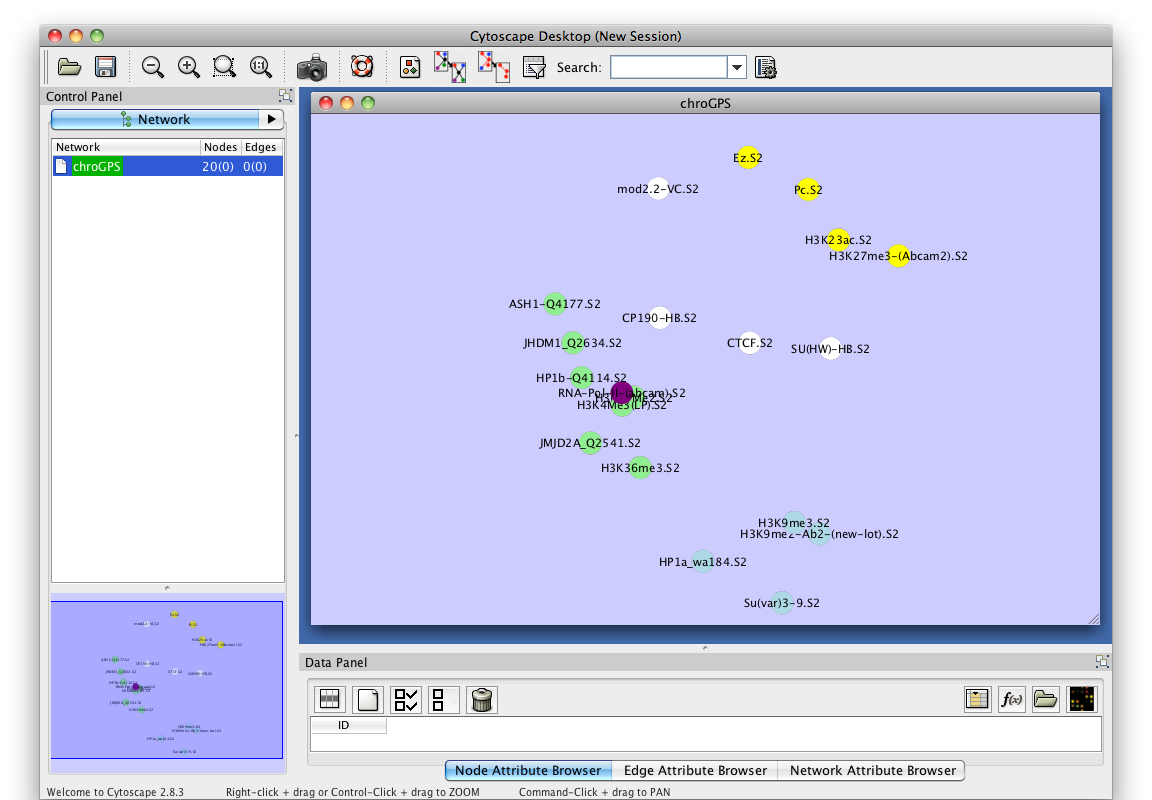
\includegraphics{chroGPS-cyto.png}}
\end{center}
\caption{chroGPS-factors network exported and visualized in Cytoscape. }
\label{fig:profile1}
\end{figure}

\normalsize

And this is everything, hope you enjoy using chroGPS as much as we did developing it !

%\bibliographystyle{plainnat}
%\bibliography{references} 

\end{document}
